\documentclass[a4paper, 14pt, twocolumn]{article}
\usepackage{xeCJK}
\usepackage{ctex}
\usepackage{graphicx}
\usepackage{listings}
\usepackage{float}
\usepackage{caption}[font=small,labelfont=bf]

\usepackage{amsmath,amsfonts,amsthm,amssymb}
\theoremstyle{definition}
\newtheorem{thm}{Theorem}
\newtheorem{exmp}{Example}
\newtheorem{defn}{Definition}
\newtheorem{lema}{Lemma}
\newtheorem{prop}{Proposition}
\newtheorem{coro}{Corollary}


\renewcommand{\baselinestretch}{1.25}


\setlength{\textwidth}{162mm}
\setlength{\textheight}{190mm}
\setlength{\textheight}{231mm}
\setlength{\headheight}{-0.1cm}
\setlength{\topmargin}{-0.1cm}
\setlength{\oddsidemargin}{-0cm}
\setlength{\evensidemargin}{-0cm}


\setlength{\parskip}{1mm}
\setlength{\unitlength}{1mm}
\setlength{\parindent}{2em}

\lstset{
    basicstyle          =   \sffamily,          % 基本代码风格
    keywordstyle        =   \bfseries,          % 关键字风格
    commentstyle        =   \rmfamily\itshape,  % 注释的风格,斜体
    stringstyle         =   \ttfamily,  % 字符串风格
    flexiblecolumns,                % 别问为什么,加上这个
%    numbers             =   right,   % 行号的位置在左边
    showspaces          =   false,  % 是否显示空格,显示了有点乱,所以不现实了
    numberstyle         =   \zihao{-5}\ttfamily,    % 行号的样式,小五号,tt等宽字体
    showstringspaces    =   false,
    captionpos          =   t,      % 这段代码的名字所呈现的位置,t指的是top上面
    frame               =   lrtb,   % 显示边框
}

\lstdefinestyle{Matlab}{
    language        =   Matlab, % 语言选Python
    basicstyle      =   \zihao{-5}\ttfamily,
    numberstyle     =   \zihao{-5}\ttfamily,
    keywordstyle    =   \color{blue},
    keywordstyle    =   [1] \color{teal},
    stringstyle     =   \color{magenta},
    commentstyle    =   \color{red}\ttfamily,
    breaklines      =   true,   % 自动换行,建议不要写太长的行
    columns         =   fixed,  % 如果不加这一句,字间距就不固定,很丑,必须加
    basewidth       =   0.5em,
}


\title{数学软件课程报告}
\author{王家蔚}
\begin{document}	
\maketitle

\section*{摘要}

这篇报告分成两个部分,第一部分是一个数据图像处理的模型,这个项目输入的是一张人像照片,输出的是人像的面部,左右眼,嘴和鼻子这几个部位的位置,并且用不同颜色把它框出来。第二部分我做的是曲面及其各处法向量的图像结果,输入的是三个等长数组,对应离散的三维点坐标,输出的是拟合出来的曲面和坐标点处的法向量。


\section{模型:人脸器官识别}
\subsection{程序结构}

\begin{figure}[H]
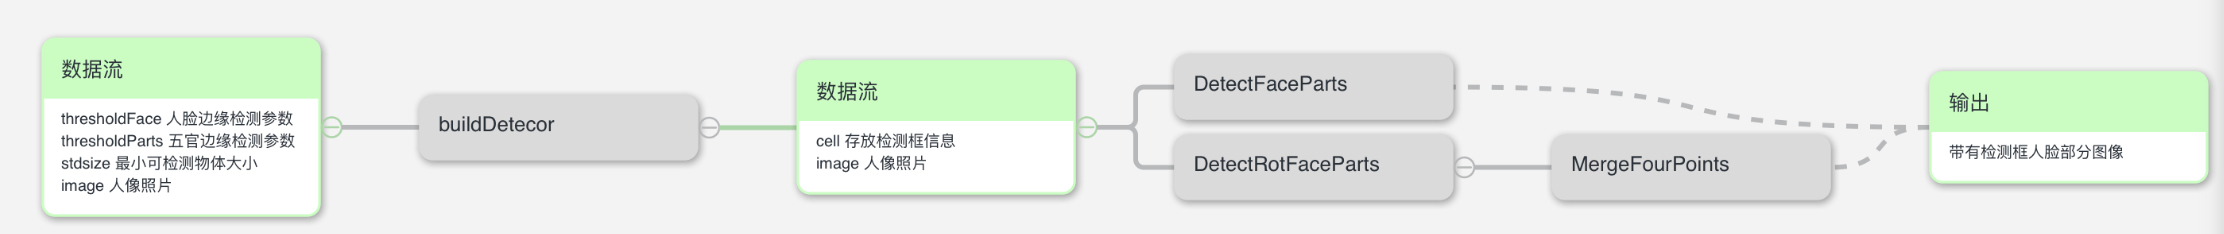
\includegraphics[width=3.1in]{process.jpeg}
\caption{程序运行流程图}
\end{figure}
简单说明一下程序设计的思路。\cite{FP D}首先输入是关于想要输出的检测框大小相关的参数,比如检测阈值和边框粗细等,这些参数通过buildDetect这个函数,转换成存储检测框信息的数据结构。这个结构再加上一张要判断的人像图片,两个数据一起输入分析五官的函数里。如果人像没有旋转,那么直接用的是DetectFaceParts函数,然后输出结果;如果人像是旋转过的,那么就要用DetectRotFaceParts这个函数,运行过程中它还会调用另外一个函数MergeFourPoints,把定位出来的四个关键位置点存放在一起,从而找到正确的方向。\\
\begin{tabular}{|c|c|c|c|}
\hline
位置 & 输入 & 位置 & 输出\\
\hline
1 & 图片 & 1 & 面部位置\\
\hline
2 & 最小搜索尺寸 & 2 &鼻子位置\\
\hline
3 & 面部阈值 & 3 & 眼睛位置\\
\hline
4 &五官阈值 & 4 &嘴巴位置\\
\hline
\end{tabular}
\\
\quad 接下来详细地介绍以下具体的实现步骤。这个程序需要用到matlab里的Image Process Package 和 Computer Vision Package,其中最核心的部分是System Object method里的step函数和vision.CascadeObjectDetector函数,后者使用的是Viola-Jones算法\cite{V-J Algo}。在旋转图像的过程中,用到的主要是maketform,得到新的图像之后再调用之前的DetectFaceParts,相当于是把图像转回去再处理。在设置参数的时候,旋转而来的图像需要设置更大的边界阈值来应对不规则的变形。
\subsection{图像结果}
为了更加客观全面地展示算法效果,我找了各国男女人像照片来进行测试,发现效果总体来说非常不错,但在局部也存在一些问题。
\begin{figure}[H]
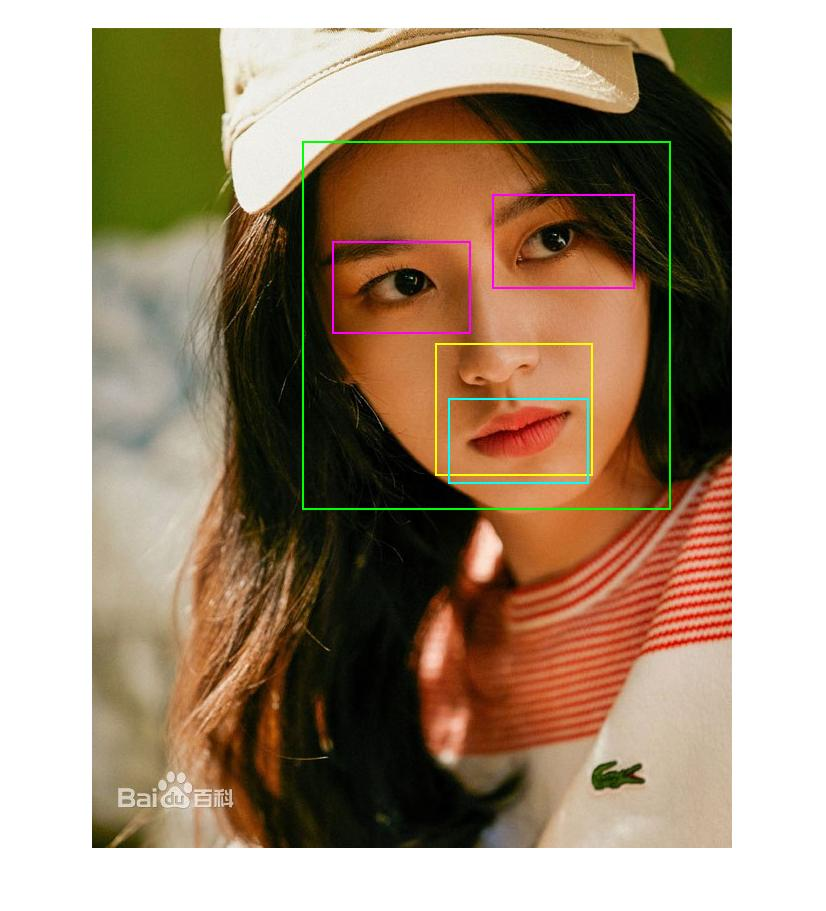
\includegraphics[width=3in]{DetectFaceParts/figure/recog1.jpg}
\caption{识别中国女性正面}
\end{figure}
比如这张照片的输出结果,显然选取鼻子的框过大,甚至包括了嘴部,但是其他部分还是非常准确的,尽管左眼有部分被头发挡住,发际线也被帽子遮住,也依然没有出现不可接受的偏差。

\begin{figure}[H]
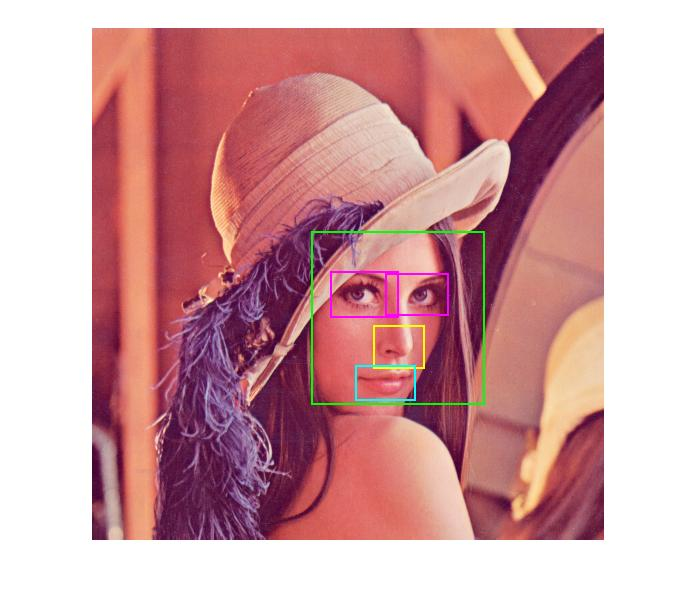
\includegraphics[width=3.5in]{DetectFaceParts/figure/recog2.jpg}
\caption{识别外国女性侧面}
\end{figure}
再用外国女像进行测试,尽管这张照片的角度更大,图像也不是很清晰,脸部占比小,但是效果更好,尤其是鼻子和嘴的重合部分明显变小了。之后的几张图片各有特点,算法都表现出极强的适应能力。
\begin{figure}[H]
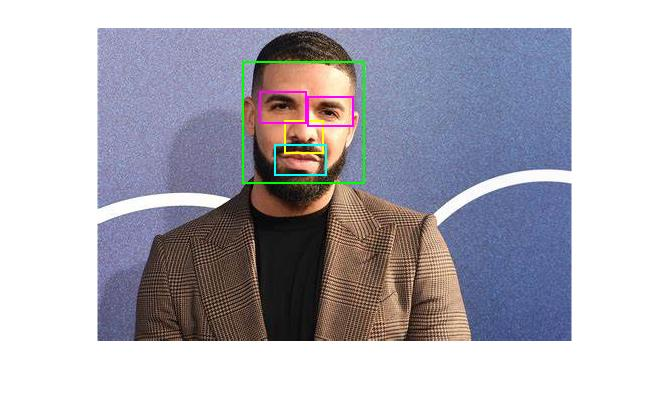
\includegraphics[width=3.5in]{DetectFaceParts/figure/recog4.jpg}
\caption{识别外国男性正面}
\end{figure}

这张照片是从正面拍摄的,而且面部的胡子很多很浓,可以发现依然存在鼻子区域过大的问题,可能是嘴唇部分的胡子影响了正常的判定。接下来测试一下有一只眼睛完全被遮住的黑人女性正面照,探究以下此时是否还能够正常识别,进而更深入地探究以下算法的识别的原理。
\begin{figure}[H]
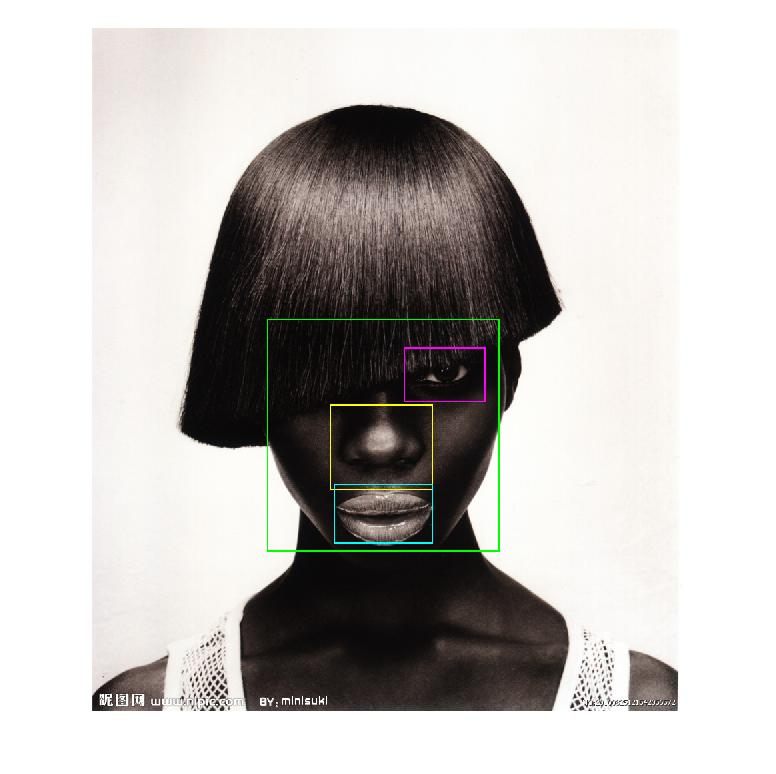
\includegraphics[width=3.5in]{DetectFaceParts/figure/recog5.jpg}
\caption{识别面部部分被遮盖}
\end{figure}
从结果上看,四个框的相对位置虽然可以辅助选择正确的区域,但并不是有了三个位置后就一定得到了第四个位置,matlab的面部识别每个部分是单独训练出来的,可以独立完成任务。
\begin{figure}[H]
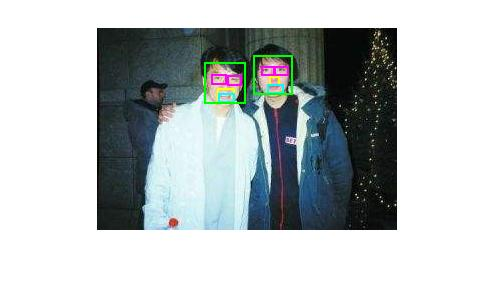
\includegraphics[width=4in]{DetectFaceParts/figure/recog6.jpg}
\caption{识别模糊的合照}
\end{figure}
这张图片里有三个人脸,但是由于我的面部识别阈值设置的稍微大了一点,所以把最后面的人忽略了,只显示出前面两个人的正面五官。尽管照片模糊,即使肉眼也很难看清,但还是精确地得到了结果。


\subsection{部分源代码}

\lstinputlisting[
    style       =   Matlab,
    caption     =   {\bf mergeFourPoints.m},
    label       =   {DFP}
    ]{DetectFaceParts/mergeFourPoints.m}
\qquad 我对这段代码改动最多,主要是重写了大量变量赋值和运算的操作,使之符合向量化和矩阵化的操作习惯,而且可以多用循环来简化代码,使它逻辑更加清晰明了。由于文件比较多,囿于篇幅不在此过多展示。
\section{模型:曲面及法向量可视化}
\subsection{程序结构}
这个项目的程序结构比较简单\cite{3d normals and curvature},首先定义三个等长数组,输入FindPointNormal函数,这个函数的核心是kd-tree算法,具体操作是先调用KDTreesearcher函数,使用欧几里得度量
\begin{equation*}
d=\sqrt{\sum_{i=1}^{n}(x_i-y_i)^2}
\end{equation*}
然后用knnsearch函数计算出相近的点。接下来,计算出协方差矩阵,为之后计算法向量和曲率作准备。最后一步,先初始化两个矩阵,一个存储曲率,另一个存储法向量,依次遍历协方差矩阵的每一个维度,根据公式
\begin{equation*}
cov(\sum_{i=1}^{n}X_i,\sum_{j=1}^{m}Y_j)=\sum_{i=1}^{n}\sum_{j=1}^{m}cov(X_i,Y_j)
\end{equation*}
\begin{equation*}
var(\sum_{i=1}^{n}X_i)=\sum_{i=1}^{n}var(X_i)+2\sum_{i,j:i<j}cov(X_i,X_j)
\end{equation*}
计算出这个维度下的协方差矩阵,然后得到这个矩阵的特征值和特征向量并存储。\\
\begin{tabular}{|c|c|c|c|}
\hline
位置 & 输入 & 位置 & 输出\\
\hline
1 & 三维点集 & 1 & 法向量\\
\hline
2 & 邻近点数量 & 2 &曲率\\
\hline
3 & 视角位置 & & \\
\hline
\end{tabular}
\qquad \qquad \qquad
为了给输出的曲面图像上色,我使用了reshape函数来把以数组形式输出的曲率变成一个方阵。我采用了quiver3函数来将向量可视化输出,并标上鲜艳的颜色。
\subsection{图像结果}
首先我们来看一个经典的例子
\begin{figure}[H]
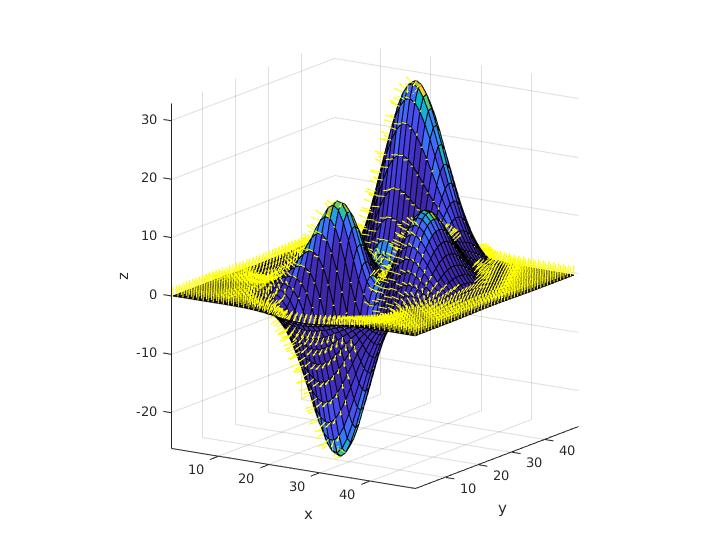
\includegraphics[width=3.5in]{FindPointNormal/figure/peak.jpg}
\caption{peak函数乘以常数倍}
\end{figure}
在demo.m文件里自定义输入的三个在最后展示图像的环节,还需要让法向量跟随视角正确显示出来,所以FindPointNormal函数的最后一个部分这就解决这个需求的。再看一个例子,
\begin{figure}[H]
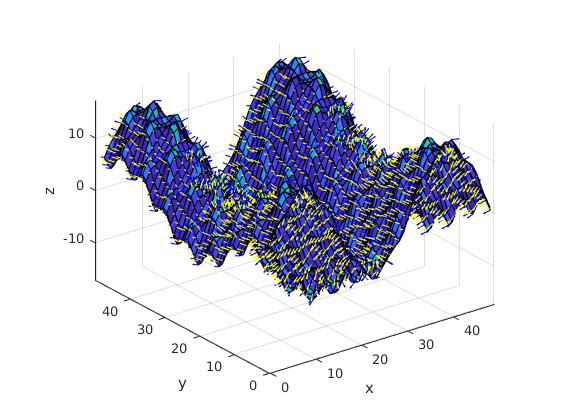
\includegraphics[width=3.5in]{FindPointNormal/figure/triangle.jpg}
\flushleft
\caption{用不同周期的正余弦构造出的函数}
\end{figure}
具体来说,这里用来生成图像的函数是
\begin{equation*}
z=10\sin{\frac{x}{5}}+5\cos{\frac{y}{7}}+\sin{x}\cos{y}
\end{equation*}
沿着x轴和y轴每一个方向都有周期性。
\subsection{部分源代码}
这段代码是程序的核心,我针对它做了很多性能上地优化,并且已经以注释的形式,把每一步想要求得的量标注了出来,在开头出给出了整体的输入和输出。值得注意的是,这里有一个输入量是可选的,而前面一个模型的每一个输入都是必须的。
\lstinputlisting[
    style       =   Matlab,
    caption     =   {\bf FindPointNormal/FindPointNormal.m},
    label       =   {DFP}
    ]{FindPointNormal/FindPointNormal.m}
\section{总结}
最后来总结一下这篇论文里我做的两个工作的,主要是想谈谈其中涉及的算法。第一个模型的核心是matlab封装好的step函数,它使用System Object实现的,经过仔细研究之后,发现它是由四个模块前后衔接而成,每个模块不仅针对图像,而且针对音频和文本都有对应的参数可以调整,值得进一步仔细研究。

第二个模型是一个几何问题,比较适合在研究比较初等的解析几何问题时,能用这程序更直观地理解正在计算的图形究竟长成什么样,帮助发现一些不太容易从解析表达式中看出来的性质。它是一个典型的利用最临近节点算法的例子,主要工作分成三步,首先是计算出样本点到其他所有点的距离,然后按照距离从近到远排序,并且选出前k个,最后少数服从多数,将这个点归并到选出的k个点中,最多的那一类里。

\begin{figure}[H]
\centering
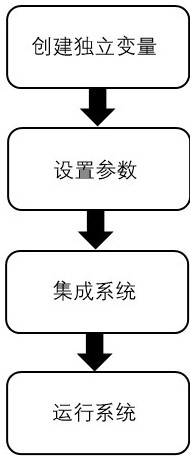
\includegraphics[width=1in]{process.jpg}
\caption{System Object运行流程}
\end{figure}

针对优化KNN算法本身,查阅资料后发现还可以尝试用不同的度量空间进行聚类操作,此外还可以不完全按照少数服从多数的原则,从全局角度来,用概率估计的方式来进行分类判定。这个算法复杂度阶数太高,对于大数据输入极度以来计算能力,可以通过改进KDTree来提高运行效率。
\begin{thebibliography}{99}
	\bibliographystyle{unsrt}
	\bibitem{FP D}Face Parts Detection,  Masayuki Tanaka 
	\bibitem{V-J Algo}Rapid Object Detection using a Boosted Cascade of Simple Features, Viola, Paul and Michael J. Jones
	\bibitem{3d normals and curvature}Find 3D Normals and Curvature, Zachary Taylor
	\bibitem{gradient}Multi-modal sensor calibration using a gradient orientation measure, Zachary Taylor

\end{thebibliography}



\end{document}
